%ajout image https://www.sharelatex.com/learn/Multi-file_LaTeX_projects

\documentclass[../rapportdestage.tex]{subfiles}

 
\begin{document}
 
 

\section{Travail réalisé}
	
	\subsection{Analyse}
		
		
		
	\begin{figure}[bh]
\centering
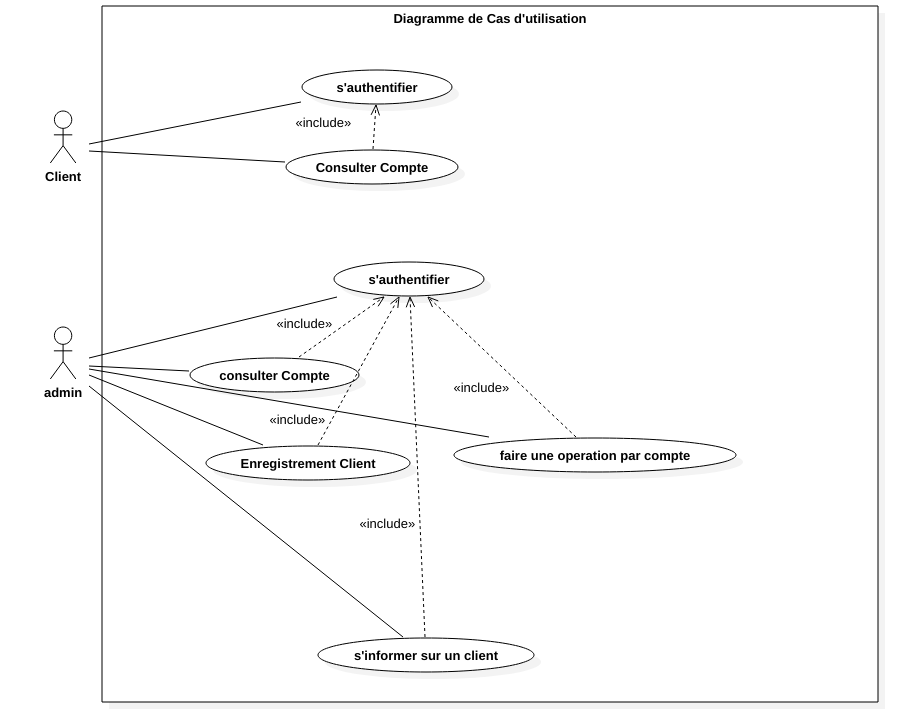
\includegraphics[scale=1.5]{DiagCasUtil.png} 
 
\label{fig:DiagrameDeCasDutilisation}
\caption{Diagramme De Cas D'utilisation}

%\end{figure}
%
%	\newpage
%	
%	
%\begin{figure}[bh]
%\centering
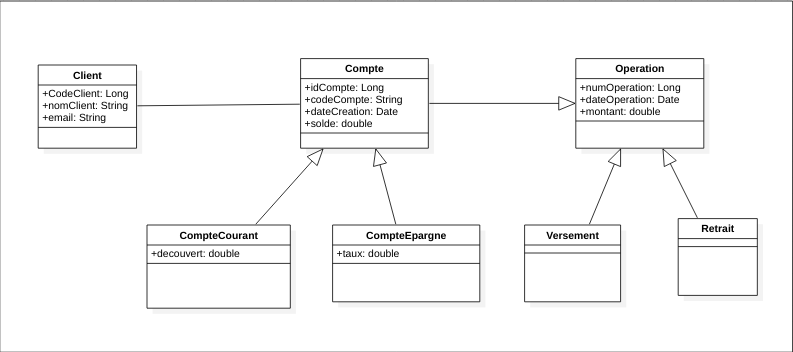
\includegraphics[scale=2]{diagclass.png} 
 
\label{fig:DiagrameDeClass}
\caption{Diagramme De Class }
\end{figure}

	\newpage
		
	
	
	
	
	\begin{figure}[bh]
\centering
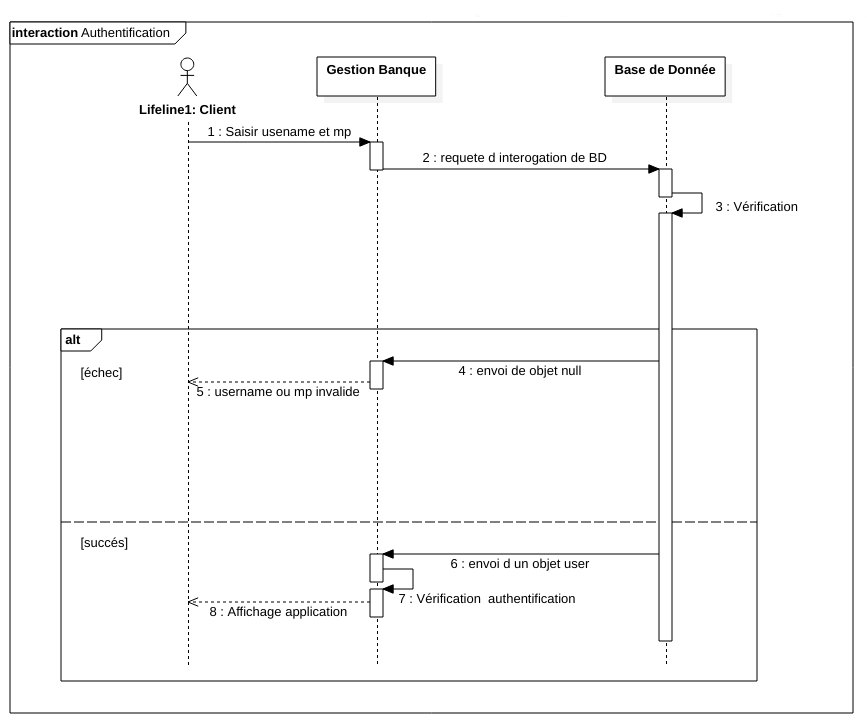
\includegraphics[scale=2]{authent.png} 
 
\label{fig:Authentification }
\caption{Diagramme de Séqunece "Authentification" }
\end{figure}
Lorsque l’utilisateur demande l’accès à l’application, il doit tout d’abord s’identifier par son identifiant et mot de passe via l’application qui prend en charge de vérifier et consulter la base de données.

S’il est accepté, donc il y’aura l’accès au système et aux applications du menu correspondant.

Sinon,un message  d’erreur est affiché afin de rectifier ses données.


\newpage


	\begin{figure}[bh]

\centering
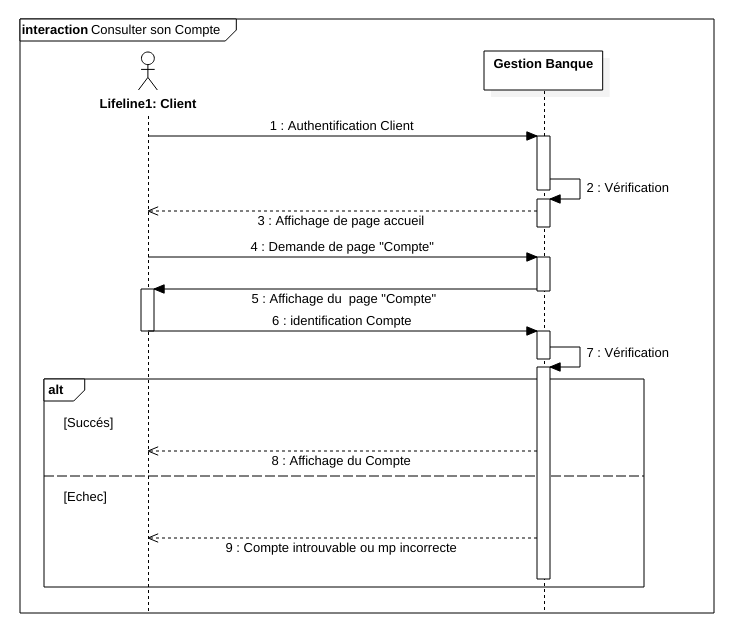
\includegraphics[scale=2]{consultercOMPTE.png}  
\label{fig:ConsulterCompte}
\caption{Diagramme De Séquence "consulter Compte" }
\end{figure}
\begin{enumerate}


\item L'utilisateur est connecté
\item La liste des comptes accessibles au client apparaît
\item Authentification du compte par mp
\item En cas de succés, pour chaque compte on a :
\begin{itemize}
\item Identifiant
\item Le solde du compte
\item Date de création
\item Le type du compte
\item Liste des opération
\end{itemize}
\end{enumerate}

	\newpage





	\begin{figure}[bh]

\centering
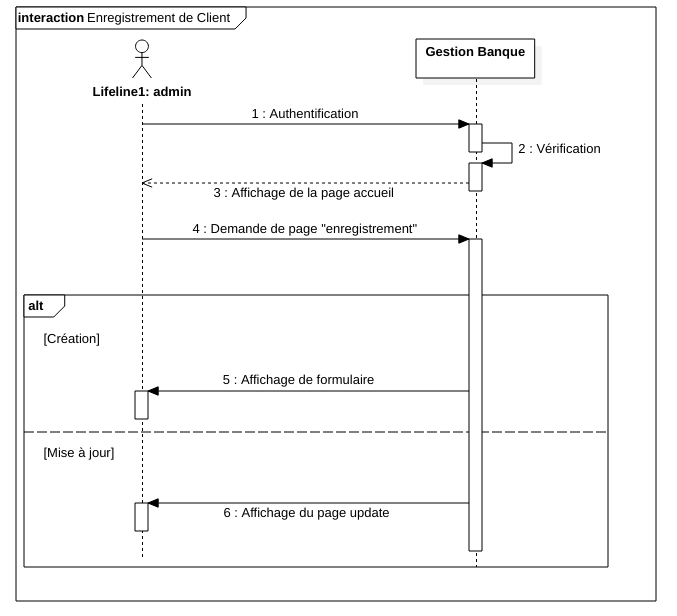
\includegraphics[scale=2]{EnregistremtnClient.png}   
\label{fig:Enregistrement d'un client}
\caption{Diagramme De Séquence "Enregistrement d'un client" }
\end{figure}

\begin{enumerate}
\item Authentification Admin
\item Accéder à la page Enregistremnt
\item Saisir les données du nouveau client
\item Validation
\end{enumerate}
	\newpage
		
	

	\begin{figure}[bh]

\centering
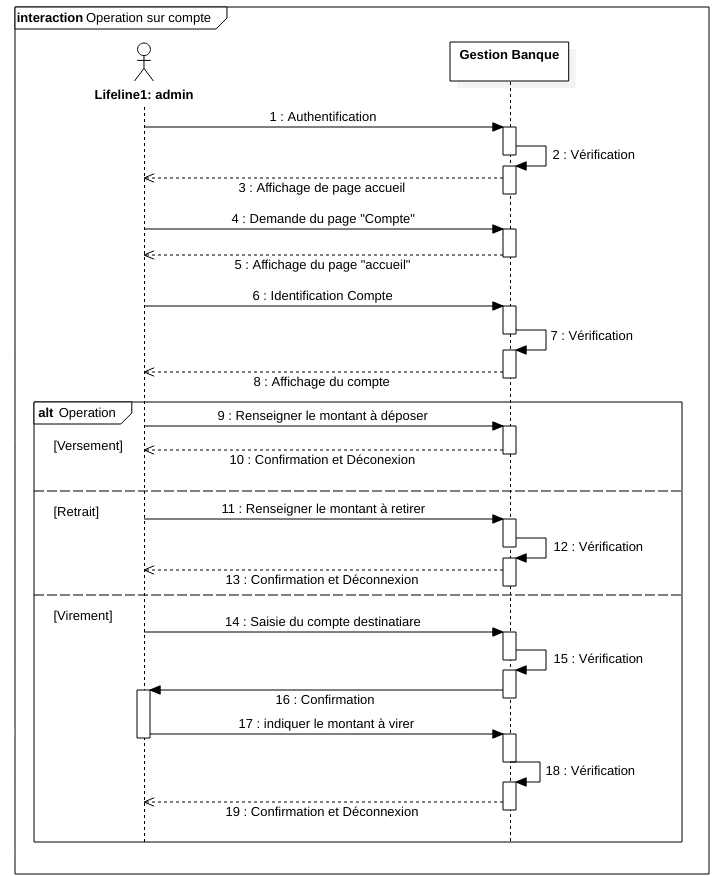
\includegraphics[scale=2]{operCompte.png} 	 
\label{fig:les Operations sur compte}
\caption{Diagramme De Séquence "opération sur Compte" }
\end{figure}
Dans le cas d'effectuer un virement:
\begin{enumerate}
\item L'utilisateur(admin) est connecté
\item Il sélectionne un compte de départ, un compte d'arrivée
\item Il fournit le montant à transférer
\item Le transfert est effectué  si le montant  le découvert maximum autorisé pour le compte à débiter. En cas d'impossibilité un message le signale à l'utilisateur
\item deconnexion
\end{enumerate}
	\newpage		 
	
	
	
	
	
		
		\subsection{Réalisation}
		
		\subsubsection{Ajout Client}
	\begin{figure}[bh]
\centering
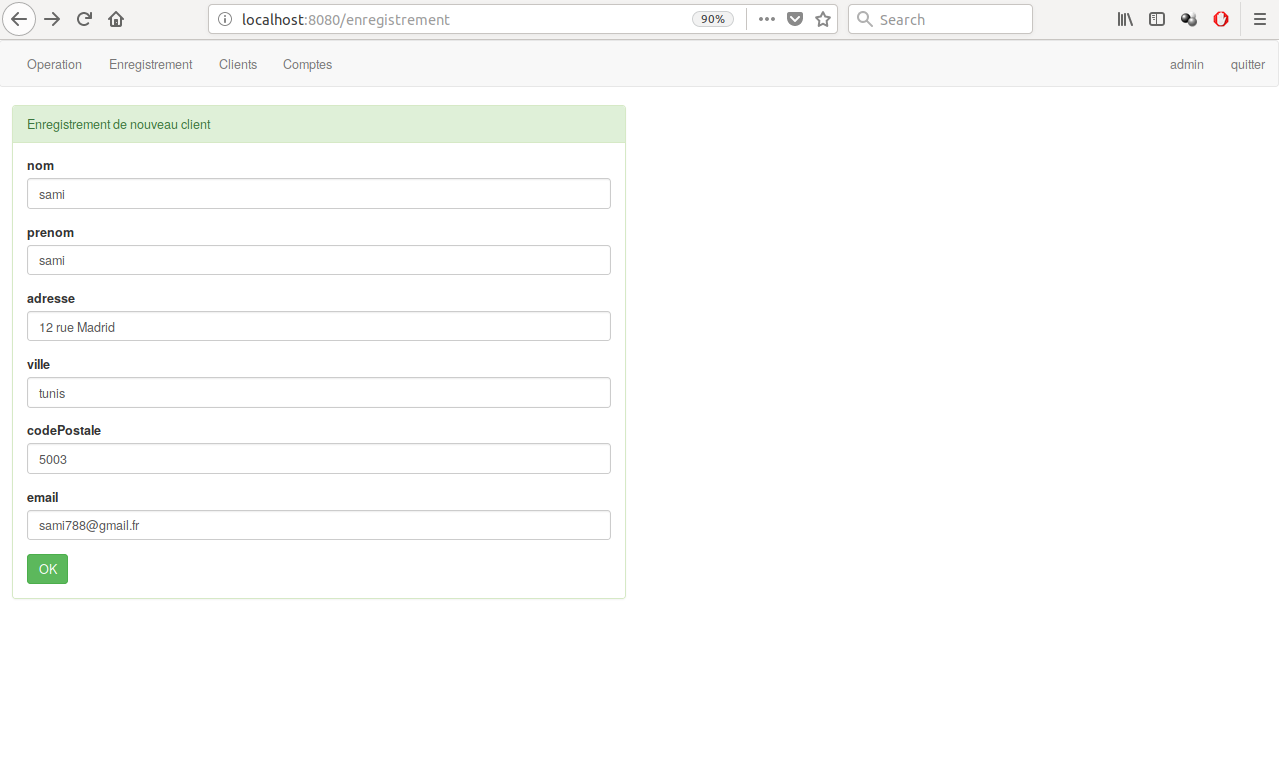
\includegraphics[scale=1.3]{enregistr.png} 
 \label{fig:Formulaire }
\caption{Formulaire }
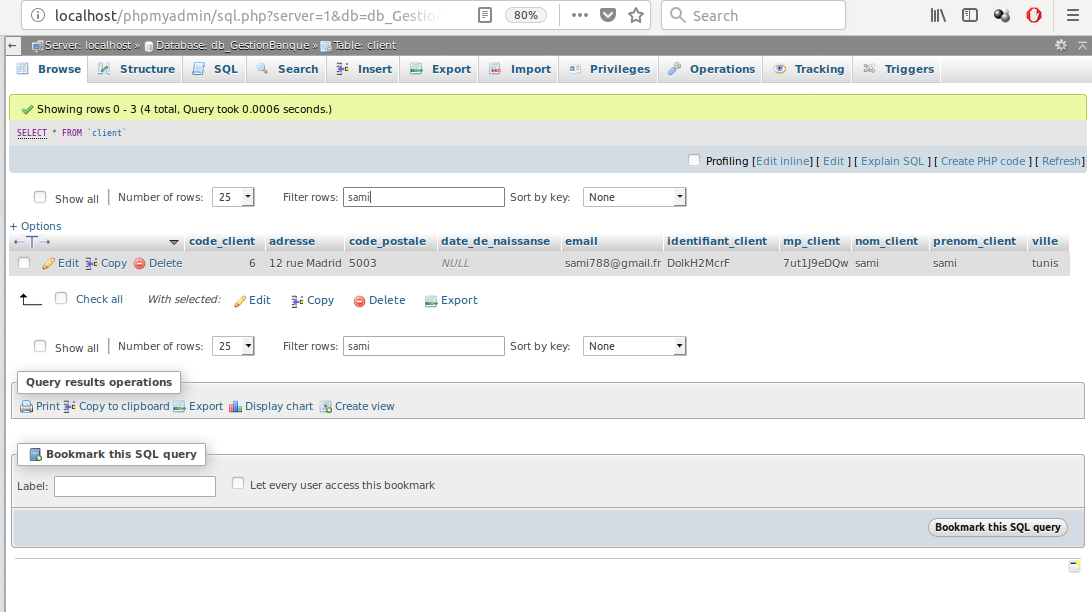
\includegraphics[scale=1.3]{enr3.png} 
 
\label{fig:Validation}
\caption{Validation }
\end{figure}
		
\clearpage
\newpage		


\subsubsection{effectuer une operation}


\begin{figure}[bh]
\centering
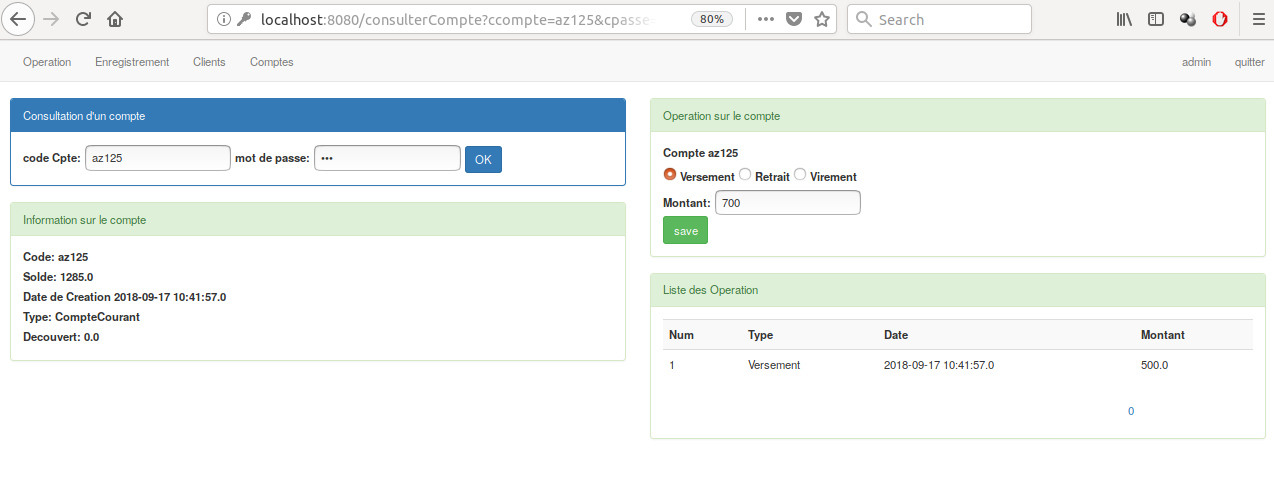
\includegraphics[scale=1.5]{compte2.png} 
 
\label{fig:Compte versement }
\caption{Compte versement}
\vspace{2cm}
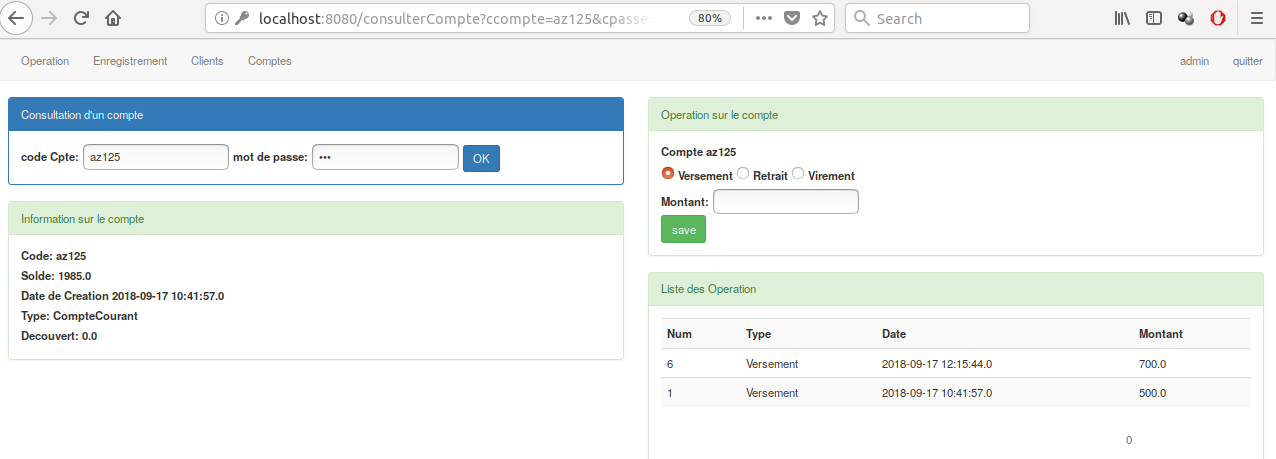
\includegraphics[scale=1.5]{compte4.png} 
 
\label{fig:Compte versement validation}
\caption{Compte versement validation}

\end{figure}
\clearpage
\newpage


\subsubsection{Information sur un compte}

\begin{figure}[bh]
\centering
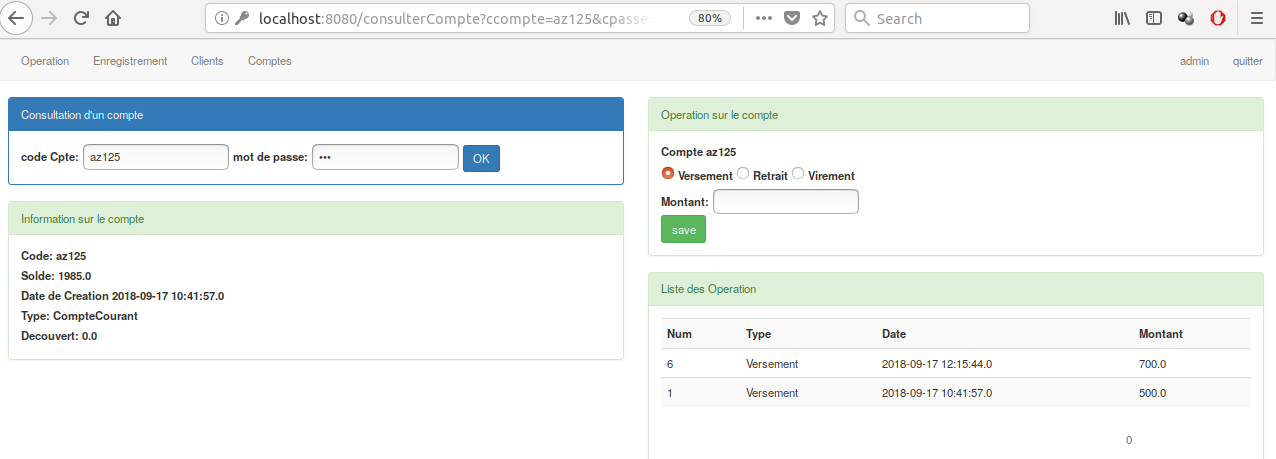
\includegraphics[scale=1.5]{compte4.png} 
 
\label{fig:Information sur un compte }
\caption{Information sur un compte}
\end{figure}




\subsubsection{Page Client}


\begin{figure}[bh]
\centering
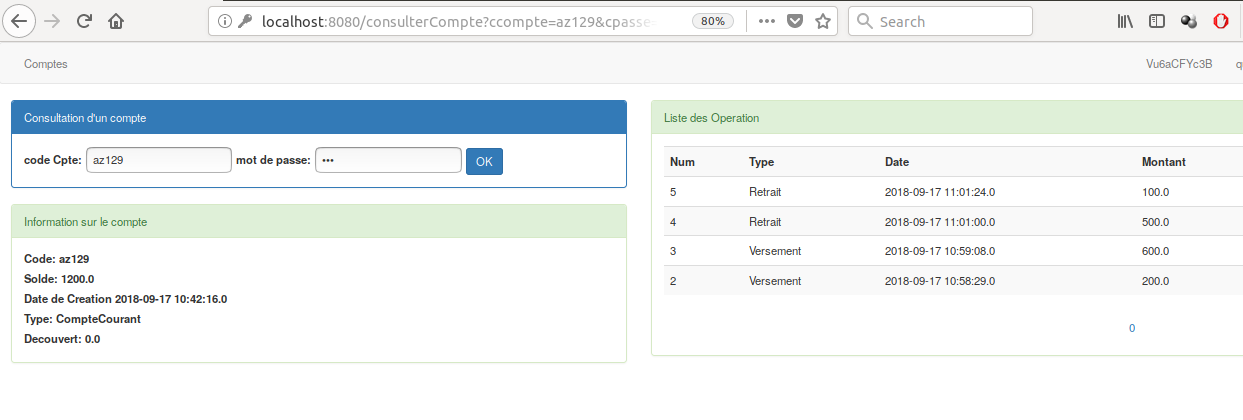
\includegraphics[scale=1.5]{cclient.png} 
 
\label{fig:Consuter son Compte }
\caption{Consulter Compte}
\end{figure}
\clearpage
\newpage
 
 
 
 
\end{document}
 





	